% ------------------------------------------------
%
%論文內容次序:
% 1.考試合格證明
% 2.中英文摘要(論文以中文撰寫者須附英文延伸摘要)
% 3.誌謝
% 4.目錄
% 5.表目錄
% 6.圖目錄
% 7.符號
% 8.主文
% 9.參考文獻
% 10.附錄
%
% 註: 參考文獻書寫注意事項:
% (1).
%    文學院之中文文獻依分類及年代順序排列。
%    其他學院所之文獻依英文姓氏第一個字母
%    (或中文姓氏第一個字筆劃)及年代順序排列。
%
% (2).
%    期刊文獻之書寫依序為:
%        姓名、文章名稱、期刊名、卷別、期別、頁別、年代。
%
% (3).
%    書寫之文獻依序為:
%        姓名、書名、出版商名、出版地、頁別、年代。
%
% ------------------------------------------------

% 封面內頁 Inner Cover
%
% 封面: 顯示所有封面內容, 沒有學校Logo
%     主要用在印刷版, 如精裝版 或 平裝版
%     (使用cover.tex來產生)
%
% 內頁: 顯示所有封面內容, 沒有學校Logo
%     主要用在電子版 + 印刷版
%
% 只要是印刷版, 不論是精裝版或平裝版, 都是 封面 (殼/皮) + 內頁.
% 只有在電子版時, 第一頁就是封面內頁.

\DisplayInnerCover

% ------------------------------------------------

% 學位考試論文證明書
\DisplayOral

% ------------------------------------------------

% 摘要 Abstract
% 除了外籍生, 本地生和僑生都是要編寫中文和英文摘要
% 論文以中文撰寫須以英文補寫 800 至 1200 字數的英文延伸摘要 (Extended Abstract)
% 詳細可看附件的學校要求或看example中的英文延伸摘要

%% ------------------------------------------------
\StartAbstractChi
% ------------------------------------------------

除了外籍生, 本地生和僑生都是要編寫中文和英文摘要. 論文以中文撰寫須以英文補寫 800 至 1200 字數的英文延伸摘要 (Extended Abstract), 如需要的話請修改`./context/abstract/extended.tex'.

外籍生則可免填中文摘要, 而在上傳時網頁資訊需填上`NONE'.\\

% ------------------------------------------------
\EndAbstractChi
% ------------------------------------------------
             % 中文版
% ------------------------------------------------
\StartAbstract
% ------------------------------------------------

Fake news has become a critical threat to information integrity and social stability, particularly in few-shot scenarios where limited labeled data is available for emerging topics or misinformation campaigns. Traditional fake news detection methods rely heavily on user propagation patterns or require extensive labeled datasets, making them impractical for real-world deployment where such data is scarce or unavailable. This thesis presents GemGNN (Generative Multi-view Interaction Graph Neural Networks), a novel framework for few-shot fake news detection that addresses these fundamental limitations through content-based graph neural network modeling.

Our approach introduces three key innovations: First, we develop a generative user interaction simulation method using Large Language Models (LLMs) to synthesize diverse user interactions with multiple tones (neutral, affirmative, skeptical), effectively overcoming the dependency on real user propagation data. Second, we propose a Test-Isolated K-Nearest Neighbor (KNN) edge construction strategy that prevents information leakage between test nodes, ensuring more realistic and robust evaluation in few-shot scenarios. Third, we implement a multi-view graph construction approach that splits news embeddings into multiple semantic perspectives, combined with multi-graph training for enhanced data augmentation.

The GemGNN framework employs Heterogeneous Graph Attention Networks (HAN) to model complex relationships between news articles and generated user interactions through dynamic attention mechanisms. Our transductive learning approach leverages both labeled and unlabeled data during message passing while restricting loss computation to labeled nodes only, maximizing the utility of limited supervision.

Extensive experiments on the FakeNewsNet datasets (PolitiFact and GossipCop) demonstrate that GemGNN significantly outperforms state-of-the-art methods across various few-shot configurations (K=3-16). Our method achieves superior F1-scores compared to traditional approaches (MLP, LSTM), transformer-based models (BERT, RoBERTa), large language models (LLaMA, Gemma), and existing graph-based methods (Less4FD, HeteroSGT). Comprehensive ablation studies validate the effectiveness of each component, showing that the combination of generative interactions, test-isolated KNN, and multi-view construction provides substantial improvements in few-shot fake news detection performance.

The contributions of this work establish a new paradigm for content-based fake news detection that eliminates dependency on user behavior data while maintaining superior performance in data-scarce scenarios, making it particularly suitable for privacy-sensitive applications and emerging misinformation detection tasks.

% ------------------------------------------------
\EndAbstract
% ------------------------------------------------
             % 英文版
%% ------------------------------------------------
\StartExtendedAbstract
% ------------------------------------------------

\ExtAbstractSummary{%
The summary is a short, informative abstract of no more than 250 words. References should not be cited. The summary should (1) state the scope and objectives of the research, (2) describe the methods used, (3) summarize the results, and (4) state the principal conclusions. Text of the summary should be 12 pt Times New Roman font, single-spaced and justified. A single line space should be left below the title `SUMMARY'. Leave a single line space above the key words listed below.
} % End of \ExtAbstractSummary{}

% ------------------------------------------------

\ExtAbstractChapter{INTRODUCTION}
The purpose of the introduction is to tell readers why they should want to read your thesis/ dissertation. This section should provide sufficient background information to allow readers to understand and evaluate the paper's results.

The introduction should (1) present the nature and scope of the problem, (2) review related literature, (3) describe the materials used and method(s) of the study, and (4) describe the main results of the study.

All text in the main body of the extended abstract should be 12 pt Times New Roman font, single-spaced and justified. Main headings are placed in the centre of the column, in capital letters using 12 pt Times New Roman Bold font. Subheadings are placed on the left margin of the column and are typed in 12 pt Times New Roman Bold font.

% ------------------------------------------------

\ExtAbstractChapter{MATERIALS AND METHODS}
There is flexibility as to the naming of the section (or sections) that provide information on the method(s) or theories employed. The methodology employed inthe work must be described in sufficient detail or with sufficient references so that the results could be duplicated.

Your materials should be organised carefully. Include all the data necessary to support your conclusions, but exclude redundant or unnecessary data.

% ------------------------------------------------

\ExtAbstractChapter{RESULTS AND DISCUSSION}
The results and discussion sections present your research findings and your analysis of those findings. The results of experiments can be presented as tables or figures.

% ------------------------------------------------

\ExtAbstractSection{Figures and Tables}
Figures may be integrated within the results section of the extended abstract, or they can be appended to the end of the written text. Figures should be black \& white. They should be no wider than the width of the A4 page.

Tables can be created within Word. As noted for figures above, if a table is to be placed within the text, it can be no wider than the width of the A4 page. Larger tables will need to be placed at the end of the abstract.

Figures and tables should be numbered according to the order they are referenced in the paper. Figures and tables should be referred to by their number in the text. When referring to figures and tables in the text, spell out and capitalize the word Figure or Table. All figures and tables must have captions.

% ------------------------------------------------

\ExtAbstractSection{Captions}
Captions should clearly explain the significance of the figure or table without reference to the text. Details in captions should not be restated in the text. Parameters in figure captions should be included and presented in words rather than symbols.

Captions should be placed directly above the relevant table and beneath the relevant figure. The caption should be typed in 12 pt Times New Roman Bold font. Spell out the word `Table' or `Figure' in full. An example table and a figure follow.

% ------------------------------------------------

\InsertTable
  [caption={Specifications of the engine}]
  {
    \begin{tabular}{llll}
    \hline
    Engine &  &  & OPEL Astra C16SE \\ \hline
    Displacement (cc) &  &  & 1598 \\
    Bore x stroke(mm x mm) &  &  & 79 x 81.5 \\
    Value mechanism &  &  & SOHC \\
    Number of valves &  &  & Intake 4, exhaust 4 \\
    Compression ratio &  &  & 9.8:1 \\
    Torque &  &  & 135/3400 Nm/rpm \\
    Power &  &  & 74/5800 kW/rpm \\
    Ignition sequence &  &  & 1-3-4-2 \\
    Spark plug &  &  & BPR6ES \\
    Fuel &  &  & 95 unleaded gasoline \\
    Cylinder arrangment &  &  & In-line 4 cylinders \\ \hline
    \end{tabular}
  } % End of  \InsertTable{}

\InsertFigure
  [scale=0.5,
    caption={HC emission as a function of equivalence ratio}]
  {./example/abstract/pic/extended-abstract-2.jpg}

% ------------------------------------------------

\ExtAbstractChapter{CONCLUSION}
This section should include (1) the main points of your paper and why they are significant, (2) any exceptions to, problems with, or limitations to your argument, (3) agreements or disagreements with previously published work, (4) theoretical and practical implications of the work, and (5) conclusions drawn.

% ------------------------------------------------
\EndExtendedAbstract
% ------------------------------------------------
        % 英文延伸摘要

% ------------------------------------------------

% 誌謝 Acknowledgments
% 誌謝正常應該只要寫一種版本就可,
% 提供2種以自行選擇所顯示的語言.
% 2種同時編寫都是可以的.

%% ------------------------------------------------
\StartAcknowledgmentsChi
% ------------------------------------------------

在這邊寫你的感謝 (對父母, 老師, 同學, 朋友等的感謝).

% ------------------------------------------------
\EndAcknowledgments
% ------------------------------------------------
             % 中文版
% ------------------------------------------------
\StartAcknowledgments
% ------------------------------------------------

Thanks someone you want in here.

% ------------------------------------------------
\EndAcknowledgments
% ------------------------------------------------
             % 英文版

% ------------------------------------------------

% 目錄 (內容, 圖表和圖片) Index of contents, tables and figures.
% 內容會自動產生 The indices will generate in automate.
\DisplayIndex                 % 顯示索引
\DisplayTablesIndex   % 顯示表格索引
\DisplayFiguresIndex  % 顯示圖片索引

% ------------------------------------------------

% Nomenclature
\StartNomChapter{Nomenclature}{chapter:nomenclature}

%%https://www.artofproblemsolving.com/wiki/index.php/LaTeX:Symbols
%https://www.sharelatex.com/learn/List_of_Greek_letters_and_math_symbols
%https://oeis.org/wiki/List_of_LaTeX_mathematical_symbols
% ------------------------------------------------

\InsertTable
  {
    \begin{tabular}{C{0.2\textwidth} L{0.4\textwidth}}
    \hline
    \underline{Symbol} & \centerline{\underline{Description}}\\
        $\alpha$ & Symbol of alpha \\
        $\beta$ & \\
        $\gamma$ & Gamma\\
    \hline
    \end{tabular}
  }

\EmptyLine

\InsertTable
  [pos=bottom, nomtitle={List of common physics notations}]
  {
    \begin{tabular}{C{0.2\textwidth} C{0.4\textwidth} C{0.35\textwidth}}
    \hline
    \underline{Symbol} & \underline{Meaning} & \underline{SI unit of measure} \\
        $g$ & Standard gravity & $9.80665 m/s^2$ \\
        $c$ & Speed of light & $\approx3.00\times108 m/s$  \\
        $l$ & Length & meter (m) \\
 	  \hline
    \end{tabular}
  }

% ------------------------------------------------

\EndNomChapter


% ------------------------------------------------

% Introduction chapter
% ------------------------------------------------
\StartChapter{Introduction}{chapter:introduction}
% ------------------------------------------------

\section{Research Background and Motivation}

In the digital age, the proliferation of fake news has emerged as one of the most pressing challenges threatening information integrity and democratic discourse. According to Vosoughi et al. \cite{vosoughi2018spread}, false news spreads six times faster than true news on social media platforms, reaching more people and penetrating deeper into social networks. This phenomenon has far-reaching consequences, from influencing electoral outcomes to undermining public health responses during critical events such as the COVID-19 pandemic.

Traditional approaches to fake news detection have relied heavily on two primary paradigms: content-based analysis and propagation-based modeling. Content-based methods analyze linguistic features, semantic patterns, and textual inconsistencies within news articles, while propagation-based approaches examine how information spreads through social networks by modeling user interactions, sharing patterns, and network topology. However, both paradigms face significant limitations in real-world deployment scenarios.

The most critical challenge in contemporary fake news detection is the few-shot learning problem, where detection systems must accurately classify news articles with minimal labeled training data. This scenario is particularly common when dealing with emerging topics, breaking news events, or novel misinformation campaigns where extensive labeled datasets are not readily available. Traditional deep learning approaches, which typically require thousands of labeled examples per class, fail to perform adequately in such data-scarce environments.

Furthermore, existing propagation-based methods, while often achieving high performance, suffer from fundamental practical limitations. These approaches require access to comprehensive user interaction data, including social network structures, user profiles, and temporal propagation patterns. Such data is increasingly difficult to obtain due to privacy regulations, platform restrictions, and the real-time nature of misinformation spread. Additionally, these methods are vulnerable to sophisticated adversarial attacks where malicious actors can manipulate propagation patterns to evade detection.

\section{Problem Statement and Challenges}

This thesis addresses the fundamental problem of few-shot fake news detection in scenarios where traditional propagation data is unavailable or unreliable. Formally, we define our problem as follows:

\textbf{Problem Definition:} Given a small set of labeled news articles $\mathcal{L} = \{(x_i, y_i)\}_{i=1}^{K \times C}$ where $K$ represents the number of examples per class and $C$ denotes the number of classes (real/fake), and a larger set of unlabeled news articles $\mathcal{U} = \{x_j\}_{j=1}^{M}$, the objective is to learn a classifier $f: \mathcal{X} \rightarrow \mathcal{Y}$ that can accurately predict labels for test instances $\mathcal{T} = \{x_k\}_{k=1}^{N}$ where $K \ll M$ and $K \ll N$.

The core challenges that motivate this research include:

\textbf{Limited Labeled Data:} Few-shot scenarios typically provide only 3-16 labeled examples per class, insufficient for training robust deep learning models using conventional approaches. This data scarcity leads to overfitting, poor generalization, and unstable performance across different domains.

\textbf{Absence of Propagation Information:} Real-world deployment often lacks access to user interaction data due to privacy constraints, platform limitations, or the time-sensitive nature of misinformation detection. Existing propagation-based methods become inapplicable in such contexts.

\textbf{Semantic Complexity:} Fake news articles often exhibit sophisticated linguistic patterns and may contain accurate factual information presented in misleading contexts. Simple content-based features fail to capture these nuanced semantic relationships.

\textbf{Domain Generalization:} Models trained on specific topics or domains often fail to generalize to emerging misinformation patterns or novel subject areas, limiting their practical applicability.

\textbf{Evaluation Realism:} Many existing few-shot learning approaches suffer from information leakage between training and test sets, leading to overly optimistic performance estimates that do not reflect real-world deployment scenarios.

\section{Research Contributions}

This thesis presents GemGNN (Generative Multi-view Interaction Graph Neural Networks), a novel framework that addresses the aforementioned challenges through several key contributions:

\textbf{Generative User Interaction Simulation:} We introduce the first approach to synthesize realistic user interactions using Large Language Models (LLMs), specifically leveraging Gemini to generate diverse user responses with multiple emotional tones (neutral, affirmative, skeptical). This innovation eliminates the dependency on real propagation data while maintaining the benefits of interaction-based modeling.

\textbf{Test-Isolated KNN Edge Construction:} We develop a novel graph construction strategy that prevents information leakage between test nodes through strict isolation constraints. This approach ensures more realistic evaluation by prohibiting test nodes from connecting to each other, addressing a critical flaw in existing graph-based few-shot learning methods.

\textbf{Multi-View Graph Architecture:} We propose a multi-view learning framework that partitions news embeddings into multiple semantic perspectives, enabling the model to capture diverse aspects of news content. Each view constructs its own graph structure, and multiple graphs are trained simultaneously to provide comprehensive data augmentation.

\textbf{Enhanced Heterogeneous Graph Neural Networks:} We design a specialized HAN-based architecture that effectively models the complex relationships between news articles and generated user interactions through type-specific attention mechanisms and hierarchical aggregation strategies.

\textbf{Comprehensive Evaluation Framework:} We establish rigorous experimental protocols that ensure fair comparison with existing methods while maintaining realistic few-shot learning constraints across multiple datasets and evaluation metrics.

\section{Thesis Organization}

The remainder of this thesis is organized as follows:

\textbf{Chapter 2: Related Work} provides a comprehensive review of existing fake news detection methods, including traditional feature-engineering approaches, deep learning techniques, graph-based methods, and few-shot learning strategies. We analyze the limitations of current approaches and position our work within the broader research landscape.

\textbf{Chapter 3: Background and Preliminaries} introduces the fundamental concepts underlying our approach, including few-shot learning formulations, graph neural network architectures, and problem notation. This chapter establishes the theoretical foundation necessary for understanding our methodology.

\textbf{Chapter 4: Methodology} presents the complete GemGNN framework, detailing the generative user interaction simulation, test-isolated KNN construction, multi-view graph architecture, and the heterogeneous graph neural network design. We provide comprehensive algorithmic descriptions and theoretical justifications for each component.

\textbf{Chapter 5: Experimental Setup} describes our experimental methodology, including dataset preprocessing, baseline method implementations, evaluation protocols, and hyperparameter configurations. We ensure reproducibility and fair comparison across all experimental conditions.

\textbf{Chapter 6: Results and Analysis} presents comprehensive experimental results, including main performance comparisons, ablation studies, and detailed analysis of model behavior. We provide insights into why our approach succeeds in few-shot scenarios and identify the key factors contributing to performance improvements.

\textbf{Chapter 7: Conclusion and Future Work} summarizes our contributions, discusses the implications of our findings, acknowledges current limitations, and outlines promising directions for future research in few-shot fake news detection.

% ------------------------------------------------
\EndChapter
% ------------------------------------------------


% Objective chapter
%% ------------------------------------------------
\StartChapter{Objective}{chapter:objective}
% ------------------------------------------------

\StartSection{起因}

做這個模版的原因其實很簡單:

\begin{enumerate}
  \item
  {
    去投國外paper時, 對方可能會要求使用LaTeX, 所以未來要懂LaTeX是不意外的.
  } % End of \item{}

  \item
  {
    想拿LaTeX來寫畢業論文, 卻發現學校只提供Mircosoft Word模版, 但卻沒有提供LaTeX的, 所以證明本模版對學校是有存在價值的.
  } % End of \item{}

  \item
  {
    因為看到發現台灣科技大學\RefBib{web:latex:template:ntust}, 台灣大學\RefBib{web:latex:template:ntu}, 元智大學\RefBib{web:latex:yzu}都能找到LaTeX的模版, 連大陸那邊都有一些學校有在提供, 更不用說國外的學校.

    那些學校的畢業論文模版不只提供是Mircosoft Word版本(.doc), 是會連LaTex(.tex)版本都有, 而我們學校卻沒有. 唯一我們學校在Google上找到的有提到的卻是數學系系網頁上的功能\RefBib{web:latex:ncku_math_introduction}和建在數學系上的一個討論區\RefBib{web:latex:ncku_math_forum}.
  } % End of \item{}

  \item
  {
    因為學校對Phd跟Master的畢業論文要求是同一個格式, 所以如果完成後對學校任何學生應該都有其好處.

    對大家都有多一個選擇來寫畢業論文, 而不是被限在使用Mircosoft Word來寫.
  } % End of \item{}

  \item
  {
    經過詢問我們資訊工程系(CSIE)的系上一些老師後, 意外發現原來某些實驗室其實已經有各自的版本存在, 但每個版本都有各自的優缺點, 例如:

    \begin{enumerate}

      \item
      {
        新的使用者或接手的人不容易修改或使用.
      } % End of \item{}

      \item
      {
        或是需要安裝的步驟十分麻煩 (e.g cwTeX\RefBib{web:latex:cwtex}).
      } % End of \item{}

      \item
      {
        另外有一些因為是只針對英文版本, 沒有考量在編寫或初稿時會有中英混雜的時候, 故這時候中英文的內容要分開編寫和產生 (學校又要求, 英文內容的論文要同時有中文論文名字等), 所以需要把整個論文分開成不同的檔案.
      } % End of \item{}
    \end{enumerate}
  } % End of \item{}
\end{enumerate}

% ------------------------------------------------

%\newpage
\StartSection{目標}
所以為了解決以上的問題, 這個模版針對了好幾點來處理:

\begin{enumerate}

  \item
  {
    把本模版做到連笨蛋都可以很快懂得使用(所謂的Books for Dummies), 所以只留下使用者要填寫的部份外, 其他都交由模版去負責.
  } % End of \item{}

  \item
  {
    希望做到使用者只讀這份模版, 就會懂得去修改和寫自己所需的內容(所謂的Self-contained. 但其實是不太可能的, 因為LaTex的使用手冊就算寫成一本幾百頁的書, 都可以缺少很多東西), 所以會同時提供很基本使用LaTex的方式, 和填寫本模版步驟.
  } % End of \item{}

  \item
  {
    希望一份模版, 能同時應用在中文或是英文版本, 只要修改內容和一些的設定.
  } % End of \item{}

  \item
  {
    把本模版open source, 讓以後任何的同學們都可以使用和修改, 以合適當時的需求.
  } % End of \item{}

\end{enumerate}

而選擇使用XeLaTex的原因, 是經過分析cwTeX, CJK和XeLaTex後. 發現cwTeX的寫法太糟, 要背多新一種語法, 而且安裝複雜\RefBib{web:latex:cwtex}; 而CJK有一定程度的設定才能在整個論文中自由使用, 感覺設定麻煩而不太能笨蛋化來用, 所以放棄選用; 故最後選用最簡單加一些包裝, 就可以簡單使用中英混合的XeLaTex.

% ------------------------------------------------

\StartSection{缺點}
但是同樣任何東西都會有缺點, 故本模版都不意外:

\begin{enumerate}

  \item
  {
    本模版是以台灣國立成功大學所最新訂下的畢業論文要求(參考: 附錄 - 撰寫論文須知 P.\RefPage{appendix:thesis-spec})來設計, 所以不一定能對非本校的人有用.
  } % End of \item{}

  \item
  {
    對沒有程式基礎, 只會用Mircosoft Word的人來講, 可能會在修改或使用上會十分吃力.
  } % End of \item{}

  \item
  {
    因為我針對某些使用者不用去接觸的部份, 進行了大量的包裝(Wrapping), 所以如果懂得LaTex的人可能會覺得我破壞了LaTex的語法. 但是本模版是針對笨蛋化和全自動, 我相信對不熟LaTex的人來講, 才不管這問題 (如同一般理論派和應用派的差別, 在意的方向完全不一樣).
  } % End of \item{}

%  \newpage
  \item
  {
    某些包裝出來的語法, 可能會在一些情況下會產生衝突而令LaTex不接受, 這時候有2種做法:
    \begin{enumerate}
      \item
      {
        不使用某些寫法, 例如已知的`\verb|\InsertFigure|'沒法被包在Table, minipage或framebox中.
      } % End of \item{}

      \item
      {
        如真的要使用那些情況, 那就不要使用模版提供的語法, 而直接去寫LaTex原版的語法.
      } % End of \item{}
    \end{enumerate}
  } % End of \item{}
\end{enumerate}

% ------------------------------------------------

\StartSection{總結}

以上是個人對這份模版的一些想法和起源, 同時希望本模版能對你提供到一些幫助.

% ------------------------------------------------
\EndChapter
% ------------------------------------------------


% Related Work chapter
% ------------------------------------------------
\StartChapter{Related Work}{chapter:related-work}
% ------------------------------------------------

Write your relatd work here.

% ------------------------------------------------
\EndChapter
% ------------------------------------------------


% Algorithm chapter
%\input{./context/algorithm/algorithm}

% Performance chapter
%\input{./context/performance/performance}

% Conclusion chapter
% ------------------------------------------------
\StartChapter{Conclusion}{chapter:conclusion}
% ------------------------------------------------

Write your conclusion here.

% ------------------------------------------------
\EndChapter
% ------------------------------------------------


% Future work chapter
%\input{./context/future-work/future-work}

% ------------------------------------------------

% 參考文獻 References
% References and bibliography

% Import the files that contain your references.
% If you set some references file,
% you need to use at least one cite to make Latex work.

\ReferencesFiles{./context/references/paper}{./context/references/misc}{./context/references/book}


% ------------------------------------------------

% 附錄 Appendix
%% ------------------------------------------------
\StartAppendix
% ------------------------------------------------

% ------------------------------------------------
\StartChapter{可使用這模版的系所}{appendix:acceptable-dept}
% ------------------------------------------------

這邊列出一些\textbf{應該可使用}或\textbf{不可使用}這模版的系所名字, 這表可能會有不正確, 所以還是先問系辦確定會比較好. \\

因為這名單都是靠網路上能找多少而得出的結果, 而如果沒有分類的話, 很高機會是使用圖書館的要求 (即是可使用本模版). \\

而如果這表名單中沒有顯示你的系所, 但你已經\textbf{知道}是否能使用, 請告知以供更新.

\clearpage

% ------------------------------------------------
\section{應該可使用}

  可使用的原因幾乎都是系所自己沒有特殊要求, 所以直接使用圖書館的要求, 而本模版就是跟隨圖書館所定下的要求來設計.

  \InsertTable
    [caption={應該可使用的系所},
      label={table:acceptable-dept:acceptable}]
    {
      \begin{tabular}{|l|l|}
      \hline
      資訊工程學系 & Department of Computer Science and Information Engineering \\ \hline
      \end{tabular}
    } % End of \InsertTable

% ------------------------------------------------
\section{應該不可使用}

  不可使用的原因是那系所已經有提供一份樣版出來, 而那份樣版的要求有沒有跟本模版一樣設計, 這個就不作詳細分析. 故如果已經有樣版, 那我就會自動把它們分類成\textit{無法使用這本模版}比較好, 但如果分類錯誤, 請告知.

  \InsertTable
    [caption={應該不可使用的系所},
      label={table:acceptable-dept:unacceptable}]
    {
      \begin{tabular}{|l|l|l|}
      \hline
      生物科技研究所 & Institute of Biotechnology & \href{www.biotech.ncku.edu.tw/files/archive/331_4b79187a.doc}{Link} \\ \hline
      體育健康與休閒研究所 & \begin{tabular}[c]{@{}l@{}}Institute of Physical Education\\ Health and Leisure Studies\end{tabular} & \href{www.ncku.edu.tw/~deprb/docs/Thesis\%20Regulation\%20.doc}{Link} \\ \hline
      \end{tabular}
    } % End of \InsertTable

% ------------------------------------------------
\EndChapter
% ------------------------------------------------

% ------------------------------------------------
\StartChapter{繳交流程說明}
% ------------------------------------------------

這部份資料來源是使用'電子學位論文服務'提供的'電子學位論文服務流程說明圖'\RefBib{web:lib:submit-flow}和'繳交論文全文電子檔案說明'\RefBib{web:lib:submit-file}.\\

\setboolean{@twoside}{false}
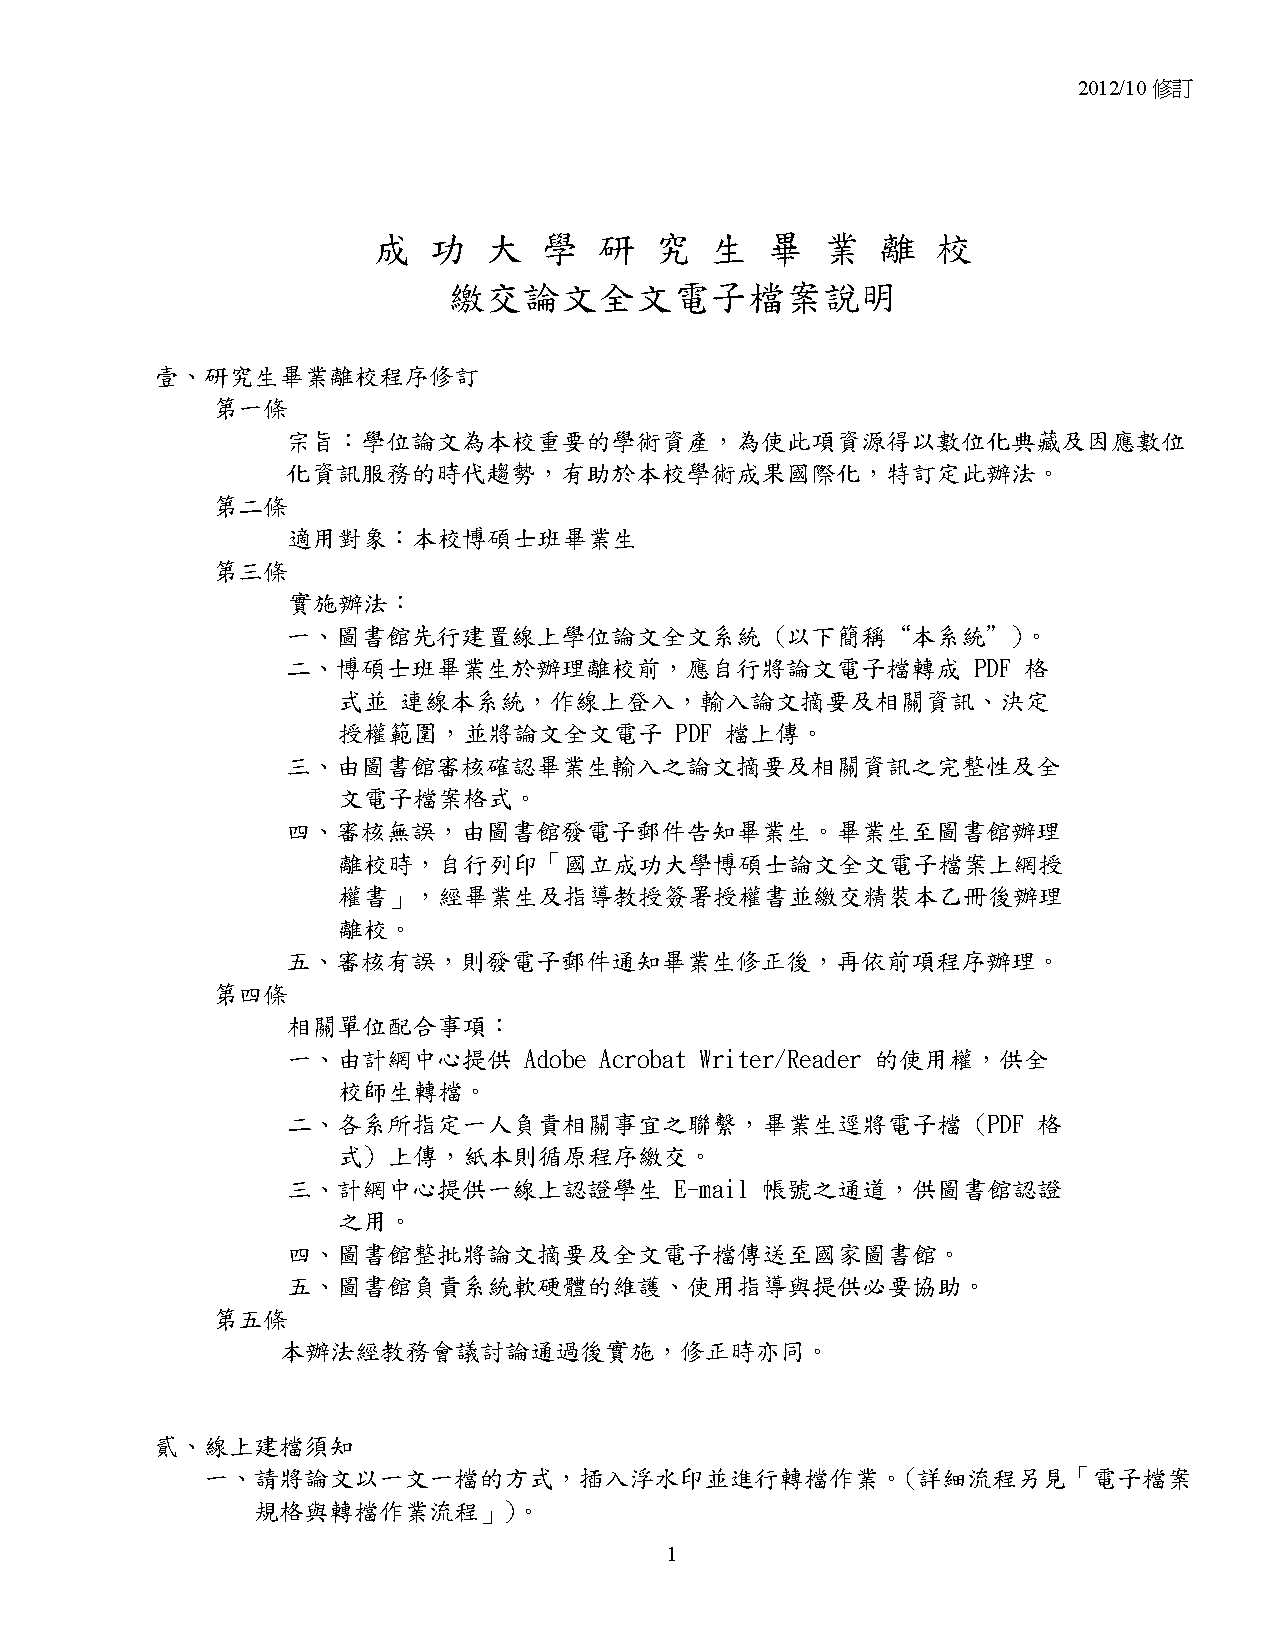
\includepdf[pages=-]{./example/appendix/pdf/2012050004-a.pdf}
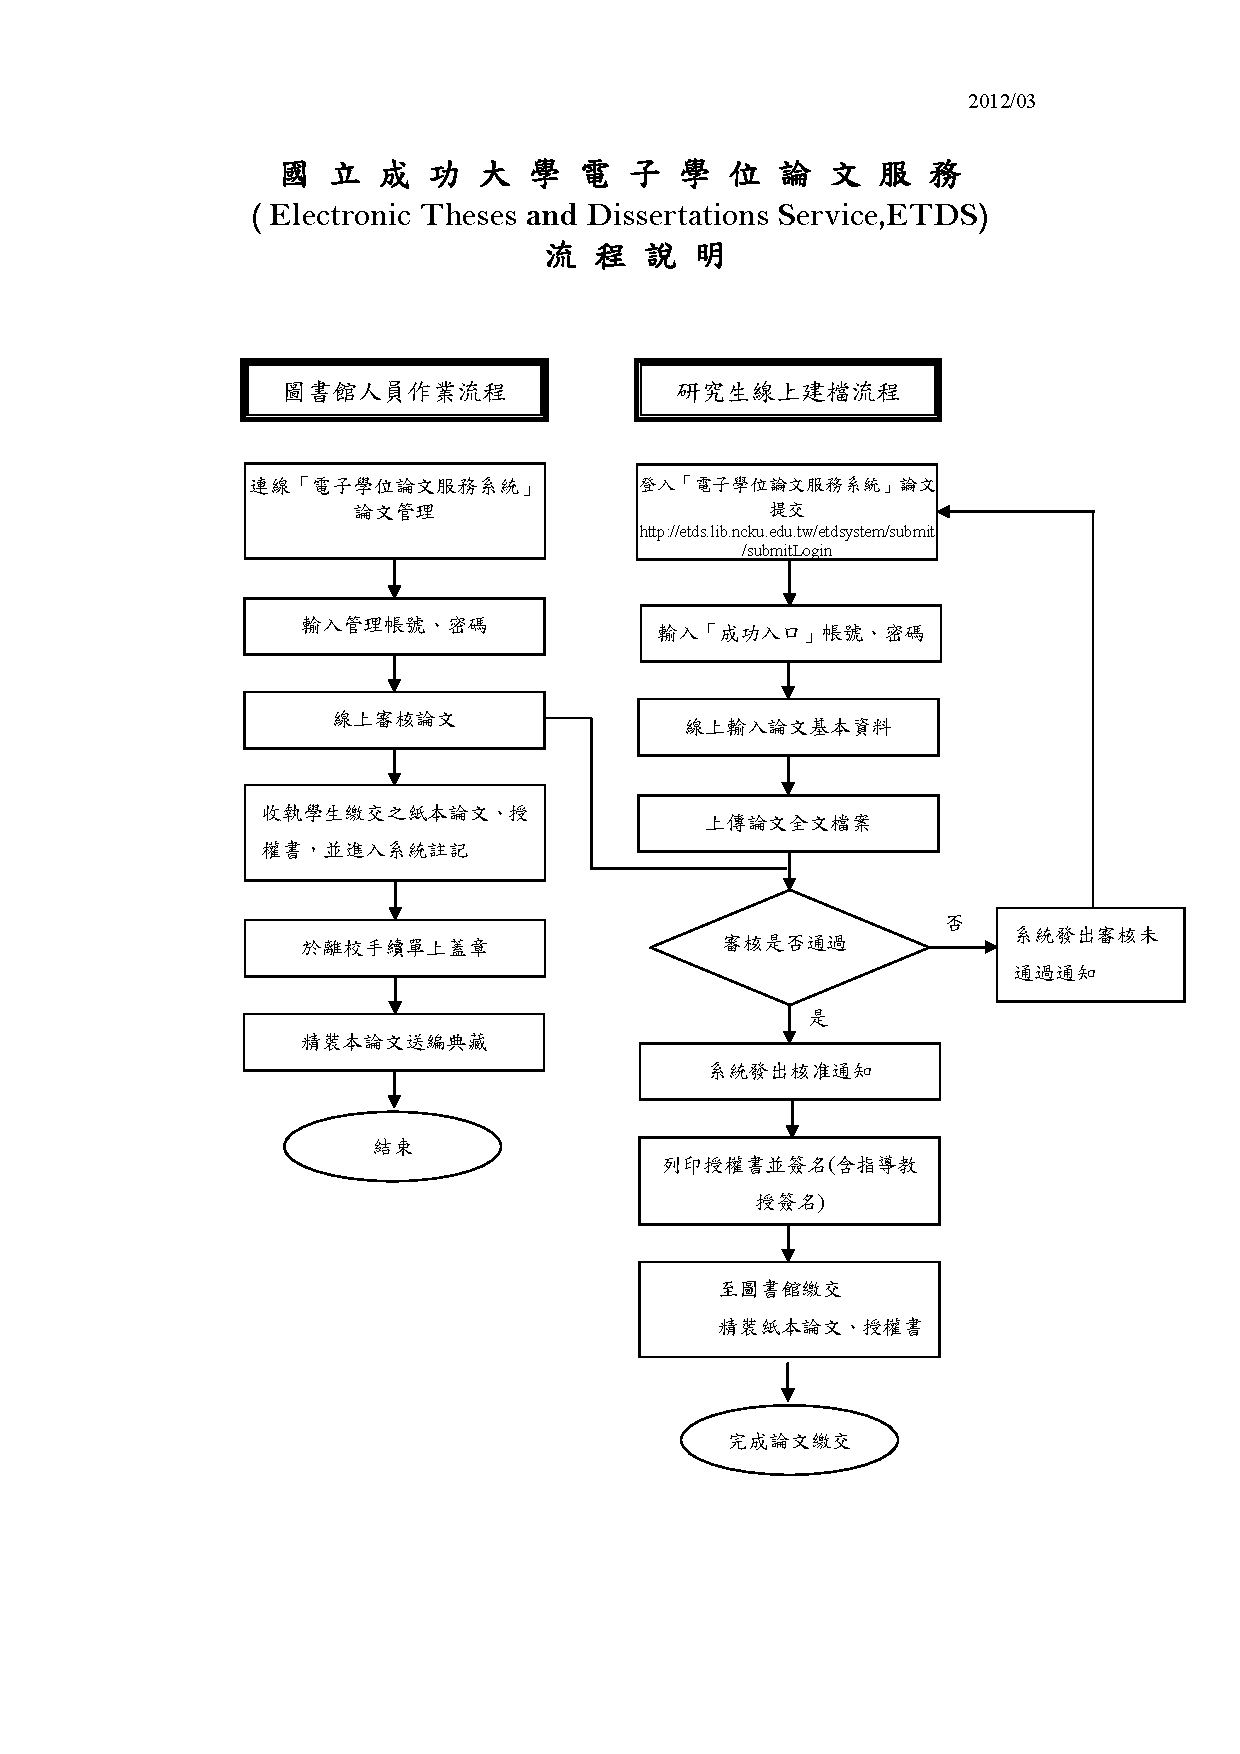
\includepdf[pages=-]{./example/appendix/pdf/2012050006-a.pdf}

% ------------------------------------------------
\EndChapter
% ------------------------------------------------

% ------------------------------------------------
\StartChapter{各系所博碩士撰寫論文須知}{appendix:thesis-spec}
% ------------------------------------------------

這部份資料來源是使用'電子學位論文服務'提供'國立成功大學博碩士學位論文格式規範'\RefBib{web:ncku:thesis-need-to-know}.\\

\setboolean{@twoside}{false}
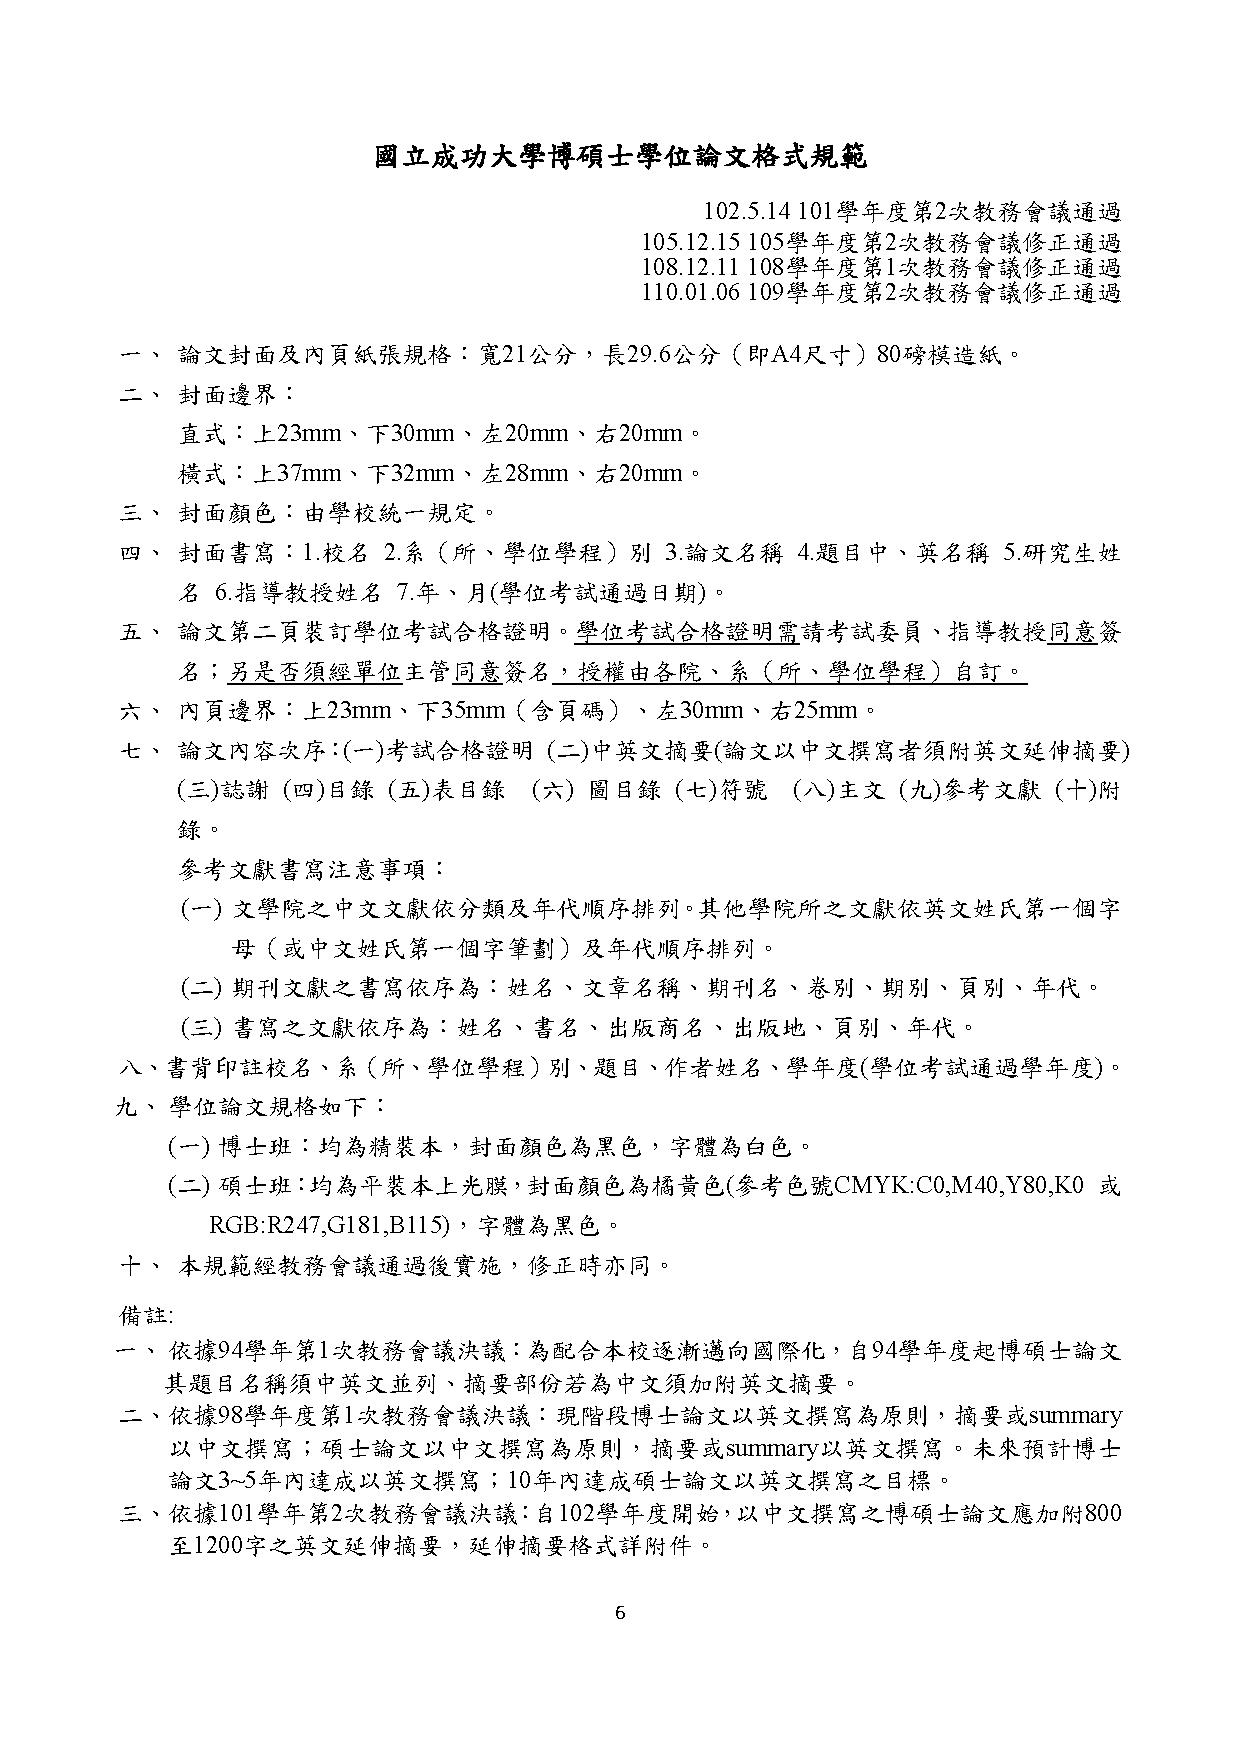
\includepdf[pages=-]{./example/appendix/pdf/thesis-spec-a.pdf}

% ------------------------------------------------
\EndChapter
% ------------------------------------------------

% ------------------------------------------------
\StartChapter{電子論文上傳前檢查事項}{appendix:e-paper_upload}
% ------------------------------------------------

這部份資料來源是使用'電子學位論文服務'中的'電子論文上傳前檢查事項'的'2012090001.pdf'\RefBib{web:lib:upload-things-check}.\\

\setboolean{@twoside}{false}
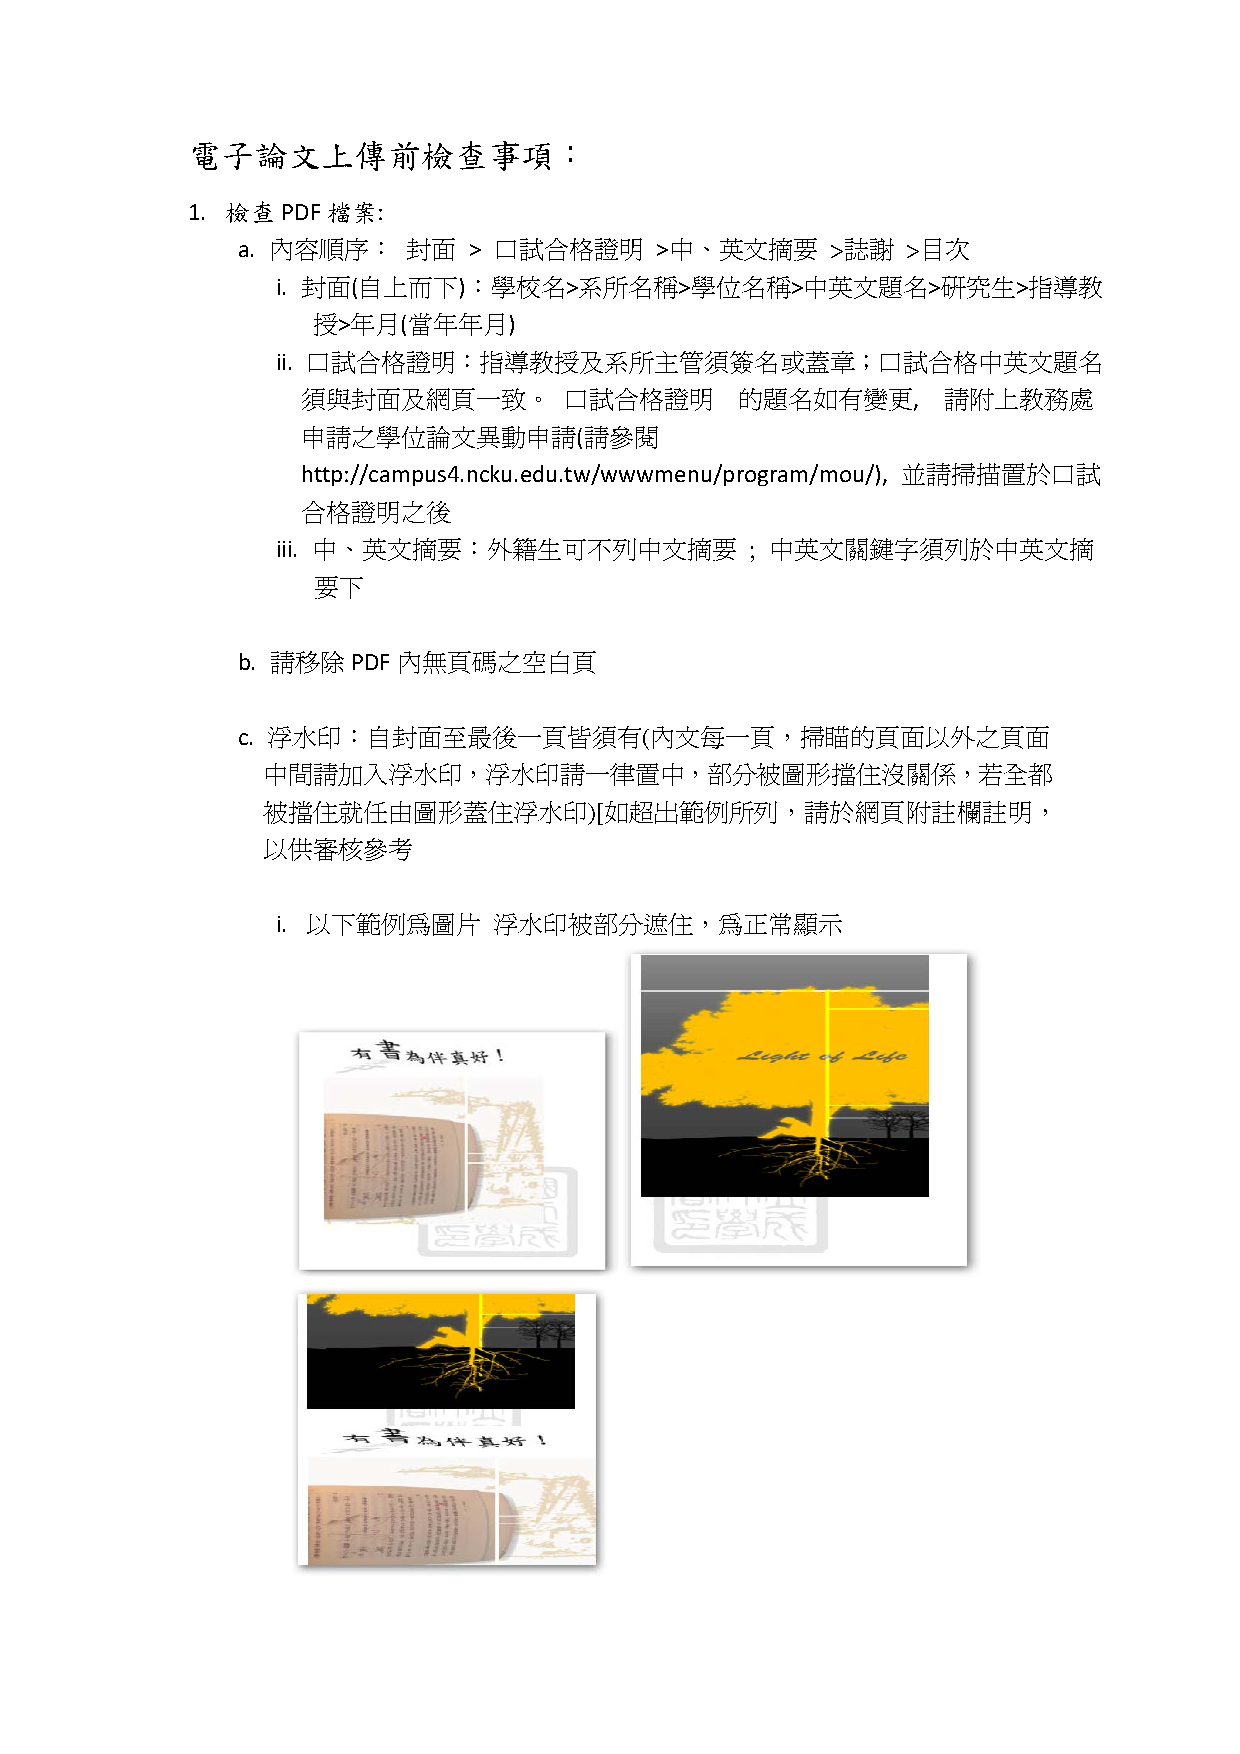
\includepdf[pages=-]{./example/appendix/pdf/2012090001-a.pdf}

% ------------------------------------------------
\EndChapter
% ------------------------------------------------

% ------------------------------------------------
\StartChapter{論文提交說明}{appendix:e-paper_upload_ppt}
% ------------------------------------------------

這部份資料來源是使用'電子學位論文服務'提供的 '2016論文提交說明簡報檔'\RefBib{web:lib:2016-submit-ppt} 修改而成的, 只抽出使用本模版後, 還要做什麼的行為.\\

\setboolean{@twoside}{false}
\includepdf[pages=-]{./example/appendix/pdf/2012050003-short-a}

% ------------------------------------------------
\EndChapter
% ------------------------------------------------

% ------------------------------------------------
\StartChapter{口試注意事項}
% ------------------------------------------------

這部份資料來源是使用本系資訊工程研究所系辦所提供的資料, 雖然內容主要針對本系, 但某些內容都是適合非本系的同學們.

\setboolean{@twoside}{false}
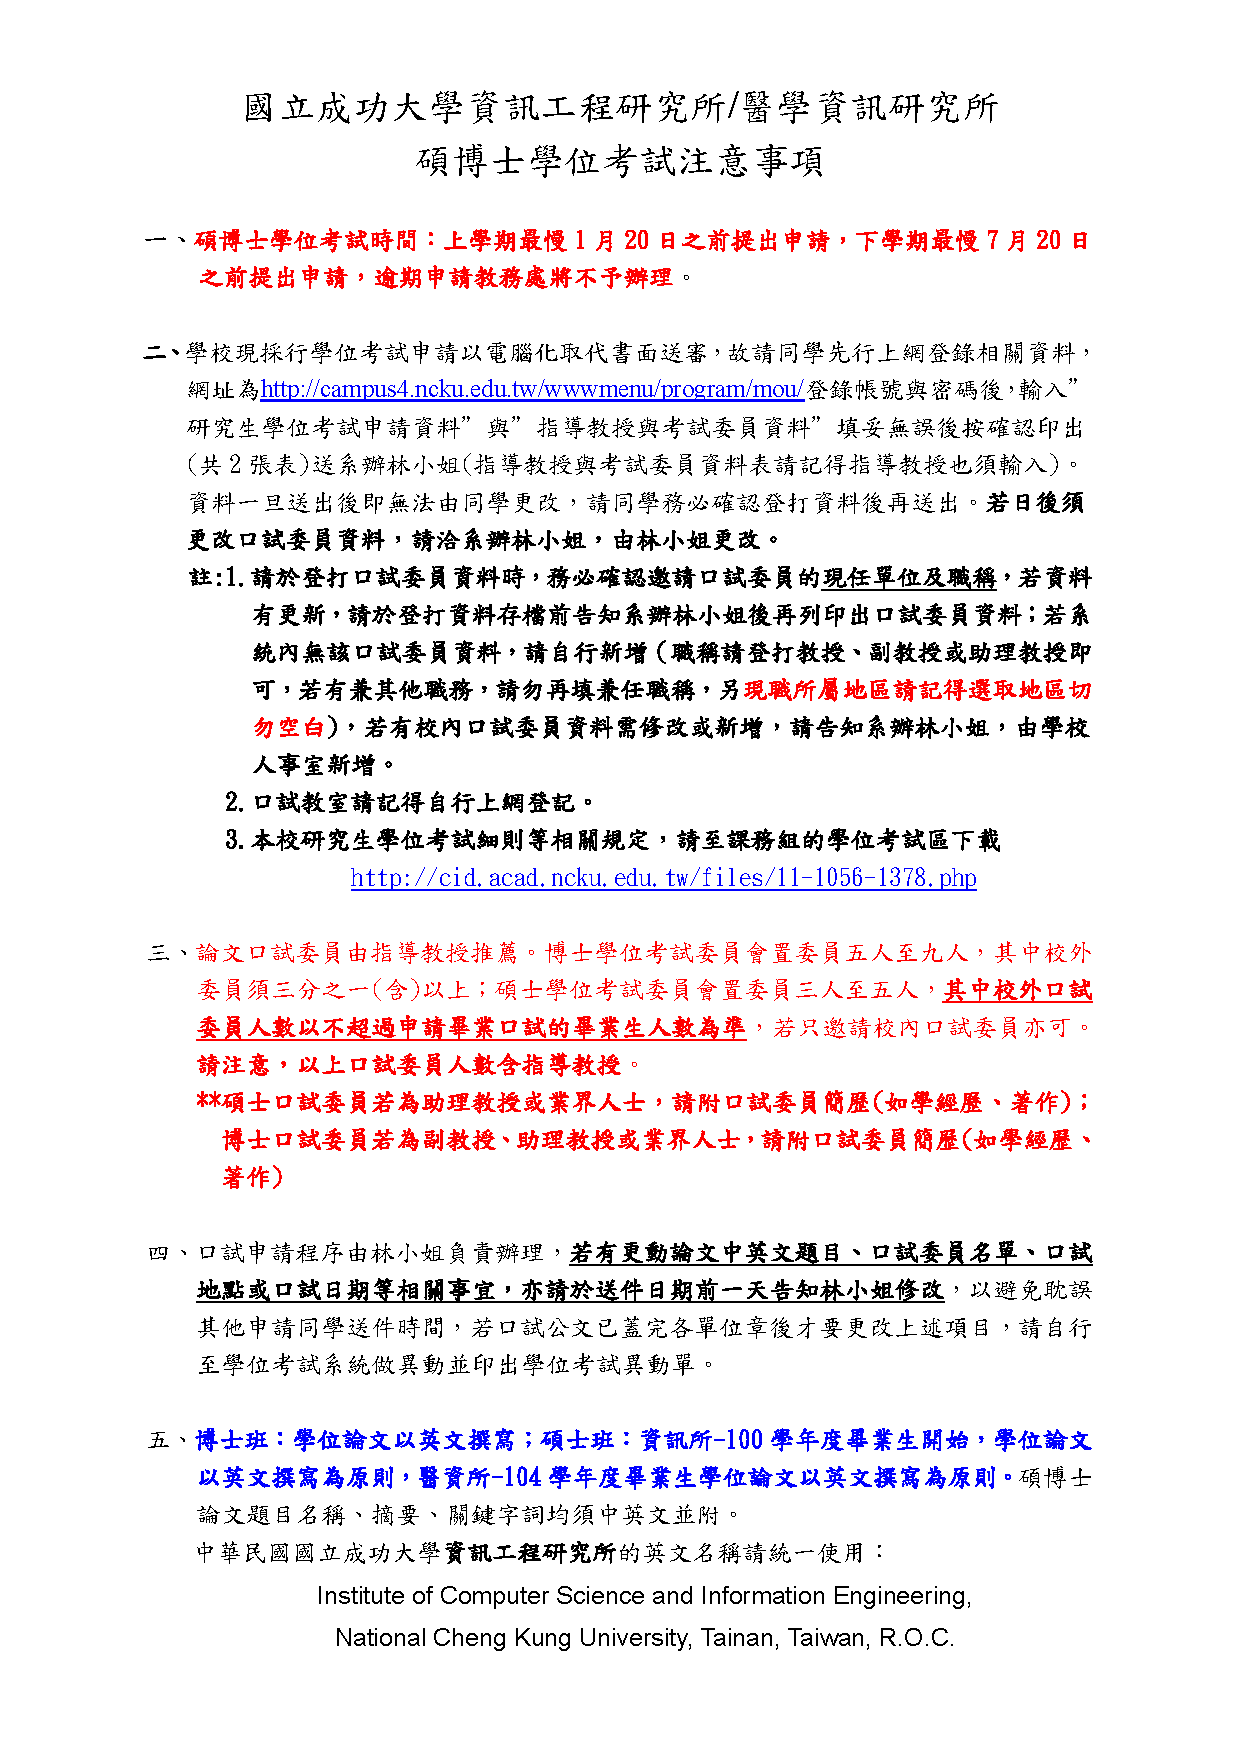
\includepdf[pages=-]{./example/appendix/pdf/oral-1040616-a.pdf}

% ------------------------------------------------
\EndChapter
% ------------------------------------------------

% ------------------------------------------------
\StartChapter{常見問題Q\&A}{appendix:faq}
% ------------------------------------------------

這部份資料來源是使用'電子學位論文服務'提供的'FAQ'\RefBib{web:lib:ETDS-QA}, 用來補充其他Appendix沒提到的一些情報.\\

\setboolean{@twoside}{false}
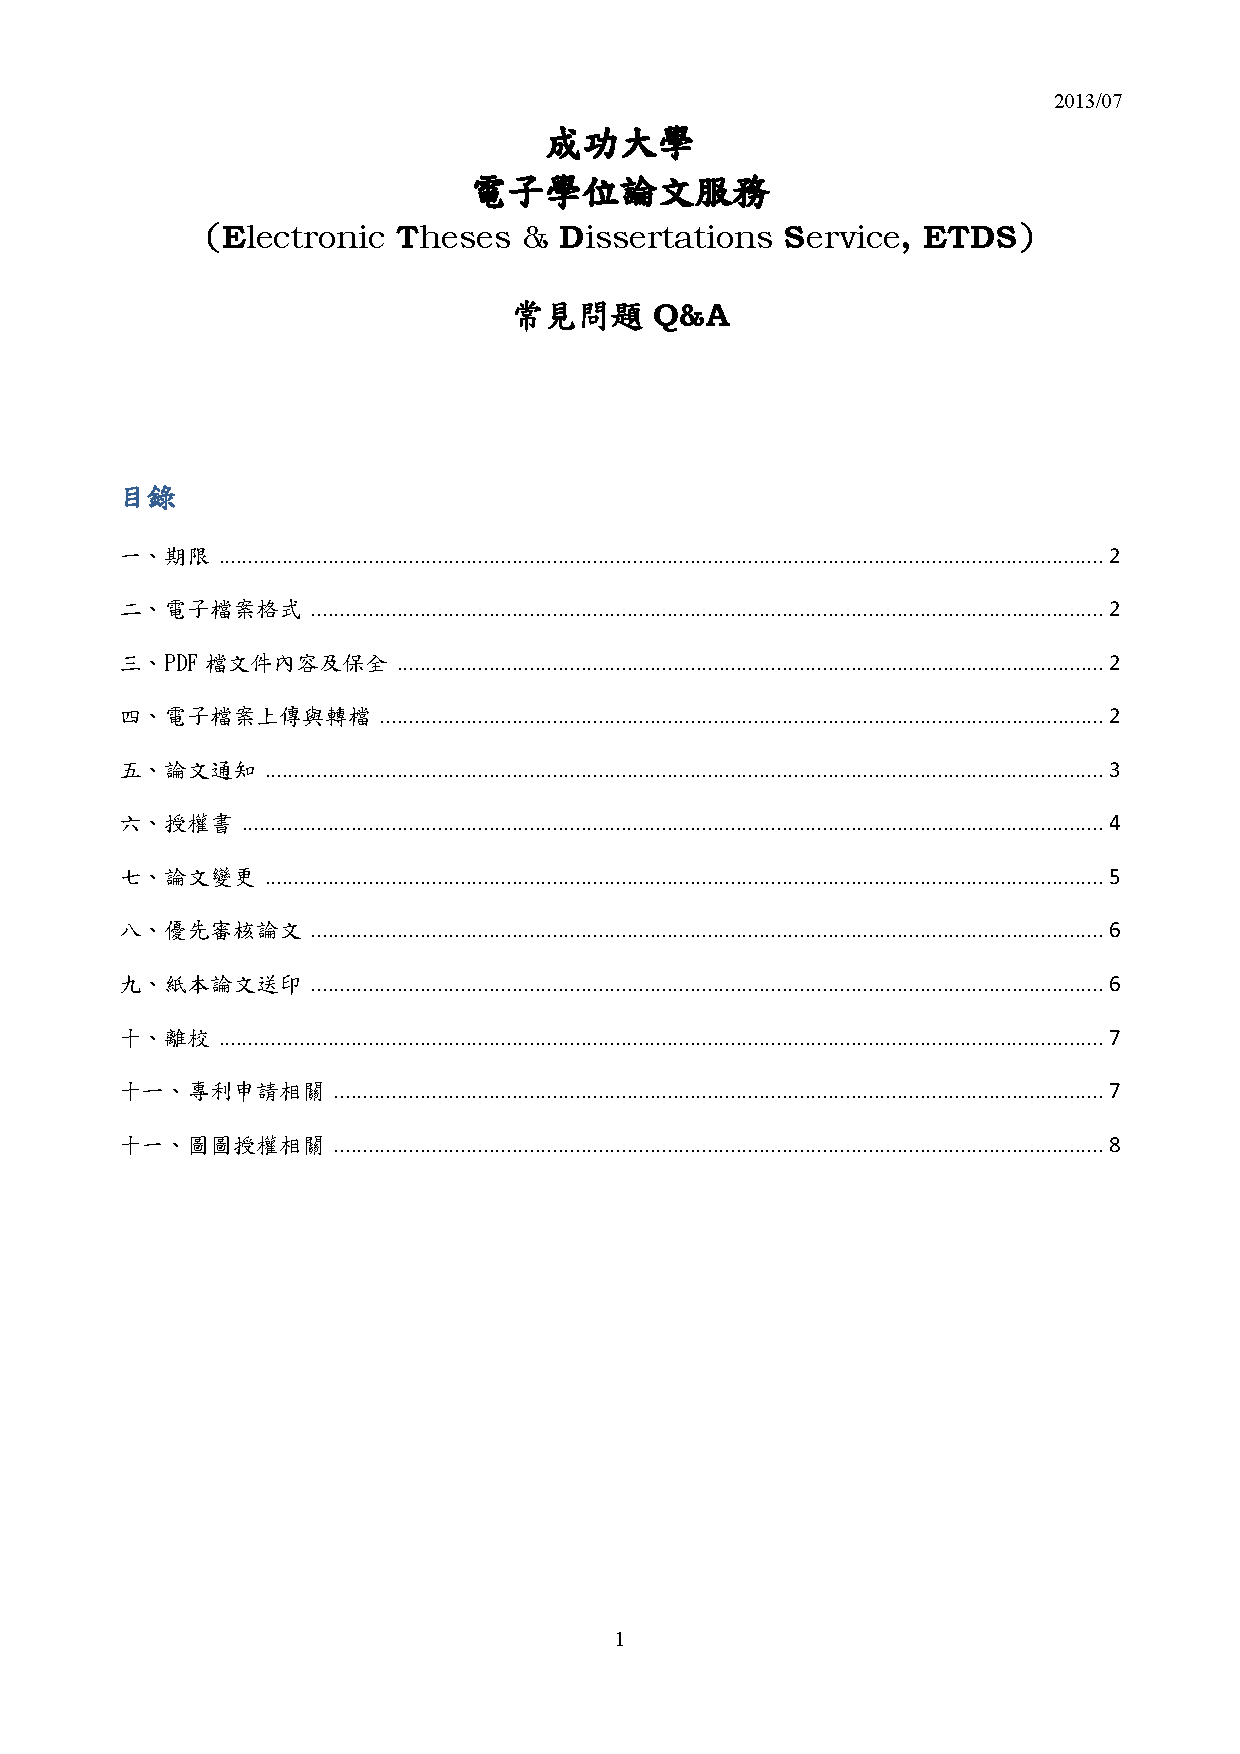
\includepdf[pages=-]{./example/appendix/pdf/2012050009-a.pdf}

% ------------------------------------------------
\EndChapter
% ------------------------------------------------

% ------------------------------------------------
\StartChapter{LaTex Symbol寫法}{appendix:unicode-symbols}
% ------------------------------------------------

這部份資料來源是xeCJK的v3.3.4(2016/02/10)版本中提供的50頁有關所有Symbol的寫法, 極度值得同學們閱讀或在這邊找你所需的Symbols.\\

內容的說明方式為:\\
Symbol: 符號所顯示的樣子\\
USV: 以Unicode方式所代表的這個符號, 例如 `(' 的Unicode寫法為U+0028.\\
Description: 是這符號的名字.\\
Macro(s): 是LaTex使用這符號的寫法.\\

\textbf{P.S: }因為符號數量多, 沒法100\%保證全能使用.

\setboolean{@twoside}{false}
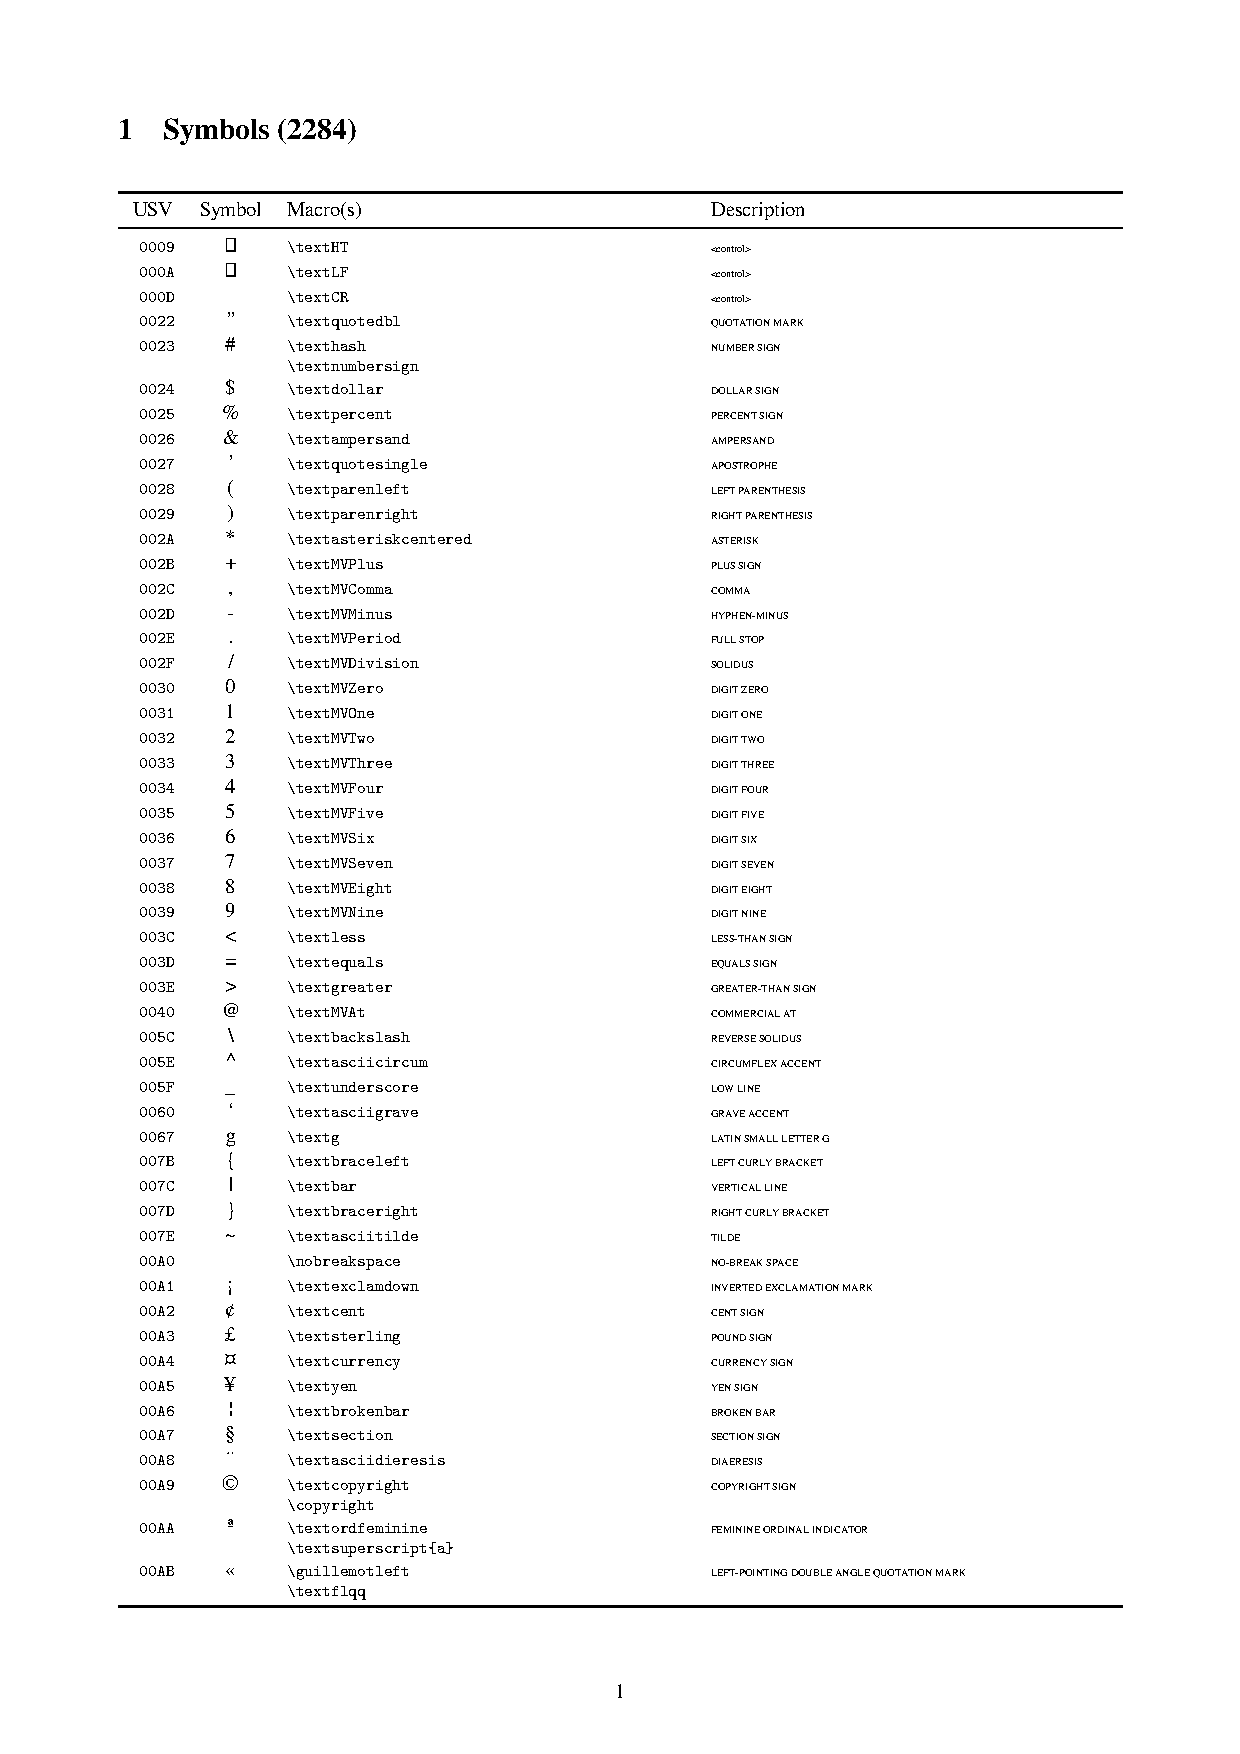
\includepdf[pages=-]{./example/appendix/pdf/xunicode-symbols.pdf}

% ------------------------------------------------
\EndChapter
% ------------------------------------------------


% ------------------------------------------------
\EndAppendix
% ------------------------------------------------


% ------------------------------------------------
